

\documentclass[bigger]{beamer}

\usepackage{style}


\title[GRIN] %optional
{A modern look at GRIN}

\subtitle{an optimizing functional language back end}

\author[P. Podlovics, Cs. Hruska ] % (optional, for multiple authors)
{Péter Podlovics, Csaba Hruska}

\institute[ELTE] % (optional)
{
	Eötvös Loránd University (ELTE), \\ Budapest, Hungary
}

\date{STCS-2019} % (optional)



\begin{document}
	
{
	\usebackgroundtemplate{
\includegraphics[width=\paperwidth]{title.jpg}}%
	\frame{\vspace{15mm}\titlepage}
}

\begin{frame}
	\frametitle{Overview}
	\tableofcontents
\end{frame}


\section{Introduction}

\begin{frame}[fragile]
	\frametitle{Why functional?}
	
	\begin{vfitemize}
		\item Declarativeness
			\begin{itemize}
				\item[pro:] can program on a higher abstraction level
			\end{itemize}
		\item Composability\\
			\begin{itemize}
				\item[pro:] can easily piece together smaller programs
				\item[con:] results in a lot of function calls
			\end{itemize}
		\item Functions are first class citizens
			\begin{itemize}
				\item[pro:] higher order functions
				\item[con:] unknown function calls
			\end{itemize}
	\end{vfitemize}

\end{frame}


\begin{frame}
\frametitle{Graph Reduction Intermediate Notation}

\begin{figure}[h]
	\centering
	\begin{adjustbox}{scale = 1.4}
		\tikzset{every loop/.style={-{Stealth[scale=1.5]}}}
		
		\begin{tikzpicture}[ node distance = 1.5cm and 1.5cm
		, on grid 
		, loop/.append style={-triangle 60}
		]
		
		\node [draw=black] (haskell)    									 {Haskell};
		\node [draw=black] (idris)   [left  =of haskell]  {Idris};
		\node [draw=black] (agda)    [right =of haskell]  {Agda};
		\node [draw=black] (grin)    [below =of haskell]  {GRIN};
		\node [draw=black] (llvm)    [below =of grin]     {LLVM};
		
		\path[-{Stealth[scale=1.5]}] 
		(idris) edge [] (grin)
		(haskell) edge [] (grin)
		(agda) edge [] (grin)
		(grin) edge [] (llvm);
		
		
		\end{tikzpicture}
	\end{adjustbox}
	\label{grin-backend}
\end{figure}
\end{frame}


\begin{frame}[fragile]
\frametitle{Front end code}

\begin{minipage}{0.35\textwidth}
	
	\begin{haskellcode}
		main = sum (upto 0 10)
		
		upto n m
		  | n > m = []
		  | otherwise = n : upto (n+1) m
		
		sum []     = 0
		sum (x:xs) = x + sum xs
	\end{haskellcode}
\end{minipage}
\hfill 
\pause
\begin{minipage}{0.4\textwidth}
	\vspace{2cm}
	\begin{figure}[h]
		\centering
		\begin{adjustbox}{scale = 1.4}
			\tikzset{every loop/.style={-{Stealth[scale=1.5]}}}
			
			\begin{tikzpicture}[ node distance = 1.3cm and 1cm
			, on grid 
			, loop/.append style={-triangle 60}
			]
			
			\node [shape=ellipse,draw=black] (main)                        {main};
			\node [shape=ellipse,draw=black] (eval) [below =of main]       {eval};
			\node [shape=ellipse,draw=black] (sum)  [below left =of eval]  {sum};
			\node [shape=ellipse,draw=black] (upto) [below right =of eval] {upto};
			
			\path[-{Stealth[scale=1.5]}] 
			(main) edge [] (eval)
			(eval) edge [bend left] (sum)
			(eval) edge [bend right] (upto)
			(sum) edge [bend left] (eval)
			(upto) edge [bend right] (eval);
			
			
			\end{tikzpicture}
		\end{adjustbox}
		\label{control-flow-lazy}
	\end{figure}
\end{minipage}
\end{frame}


\begin{frame}[fragile]
\frametitle{GRIN code}

\begin{minipage}{0.4\textwidth}
	
	\begin{haskellcode}
		grinMain = 
		  t1 <- store (CInt 1)
		  t2 <- store (CInt 10)
		  t3 <- store (Fupto t1 t2)
		  t4 <- store (Fsum t3)
		  (CInt r) <- eval t4
		  _prim_int_print r
	\end{haskellcode}
\end{minipage}
\hfill
\begin{minipage}{0.48\textwidth}
	\vspace{1cm}
	\begin{haskellcode}
		eval p = 
		  v <- fetch p
		  case v of
		    (CInt n)     -> pure v
		    (CNil)       -> pure v
		    (CCons y ys) -> pure v
		    (Fupto a b) -> 
		      zs <- upto a b
		      update p zs
		      pure zs
		    (Fsum c) -> 
		      s <- sum c
		      update p s
		      pure s
	\end{haskellcode}
\end{minipage}


\end{frame}


\begin{frame}[fragile]
\frametitle{Transformation machinery}

	\begin{vfitemize}
		
		\item Inline calls to \mintinline{haskell}{eval}
		\item Run dataflow analyses:
			\begin{itemize}
				\item Heap points-to analysis
				\item Sharing analysis
			\end{itemize}
		\item Run transformations until we reach a fixed-point:
			\begin{itemize}
				\item Sparse Case Optimization
				\item Common Subexpression Elimination
				\item Generalized Unboxing
				\item etc \dots
			\end{itemize}
		
	\end{vfitemize}


\end{frame}


\section{Extensions}

\begin{frame}[fragile]
\frametitle{Extending Heap points-to}

	\vspace{1cm}
	\begin{minipage}{\textwidth}
		\begin{figure}
			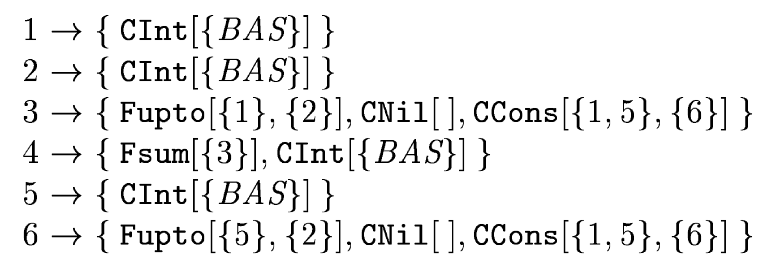
\includegraphics[scale=0.3]{hpt-boq.png}
		\end{figure}
	\end{minipage}
	\vfill
	\pause
	\begin{minipage}{\textwidth}
		\begin{figure}
			$BAS \in \{ \text{Int64}, \text{Float}, \text{Bool}, \text{String}, \text{Char} \}$
		\end{figure}
	\end{minipage}
	\vfill
	\pause
	\begin{center}
		\begin{minipage}{0.8\textwidth}
			% real type would be: a -> State# s -> (# State# s, MutVar# s a #)
			\begin{haskellcode}
				indexArray# :: Array# a -> Int# -> (# a #)
				newMutVar#  :: a -> s -> (# s, MutVar# s a #)
			\end{haskellcode}
		\end{minipage}
	\end{center}

\end{frame}


\begin{frame}[fragile]
\frametitle{LLVM back end}

	\hspace{-4cm}
	\begin{minipage}[t]{0.30\textwidth}
		\begin{minted}[fontsize=\scriptsize]{haskell}		
			grinMain =
			 t1 <- store (CInt 1)
			 t2 <- store (CInt 10)
			 t3 <- store (Fupto t1 t2)
			 t4 <- store (Fsum t3)
			 (CInt r') <- eval t4
			 _prim_int_print r'
			 
			upto m n =
			 (CInt m') <- eval m
			 (CInt n') <- eval n
			 b' <- _prim_int_gt m' n'
			 case b' of
			   #True -> pure (CNil)
			   
			sum l = ...
			
			eval p = ...
		\end{minted}
	\end{minipage}
	\hspace{1.8cm}
	\pause
	\begin{minipage}[t]{0.30\textwidth}
		\begin{minted}[fontsize=\scriptsize]{haskell}
		grinMain =
		 n1 <- sum 0 1 10
		 _prim_int_print n1
		
		sum s lo hi =
		 b <- _prim_int_gt lo hi
		 if b then
		  pure s
		 else
		  lo' <- _prim_int_add lo 1
		  s' <- _prim_int_add s lo
		  sum s' lo' hi

		\end{minted}
	\end{minipage}
	\hspace{0.5cm}
	\pause
	\begin{minipage}[t]{0.30\textwidth}
		\begin{minted}[fontsize=\scriptsize]{asm}
		grinMain:                      
		# BB#0:                     
		  movabsq    $55, %rdi  
		  jmp    _prim_int_print       
		\end{minted}
	\end{minipage}

\end{frame}
%$

\section{Dead Data Elimination}

\begin{frame}[fragile]
\frametitle{Dead data elimination}

\begin{center}
	\begin{minipage}{0.30\textwidth}
		\begin{haskellcode}
			length : List a -> Nat
			length Nil = Z
			length (Cons x xs) 
			  = S (length xs)
		\end{haskellcode}
	\end{minipage}
	\hspace{1cm}
	$\xRightarrow{\text{DDE}}$
	\hfill
	\begin{minipage}{0.5\textwidth}
		\begin{haskellcode}
			length p =
			 xs <- fetch p
			 case xs of
			  (Cons ys) ->
			   l1 <- length ys
			   l2 <- _prim_int_add l1 1
			   pure l2
			  (Nil) ->
			    pure 0
		\end{haskellcode}
	\end{minipage}
\end{center}


\end{frame}

\begin{frame}
\frametitle{Applications}

	\begin{vfitemize}
		\item Map $\rightarrow$ Set
		\item Type class dictionaries
		\item Type erasure for dependently typed languages
	\end{vfitemize}

\end{frame} 

\begin{frame}
\frametitle{What do we need?}

	\begin{vfitemize}
		\item Producers \& consumers
		\item Detect dead fields
		\item Connect consumers to producer
		\item Remove or transform dead fields
	\end{vfitemize}

\end{frame}

\begin{frame}[fragile]
\frametitle{Created-by}

\begin{center}
	\begin{minipage}{0.4\textwidth}
		\begin{haskellcode}
			grinMain =
			  a0 <- pure 5
			  n0 <- pure (CNil)
			  p0 <- store n0 
			  n1 <- pure (CCons a0 p0)
			  r  <- case n1 of 
			    (CNil) -> 
			      pure (CNil)
			    (CCons x xs) -> 
			      xs' <- fetch xs
			      pure xs'
			  pure r
		\end{haskellcode}
	\end{minipage}
	\hfill
	\begin{minipage}{0.40\textwidth}
		\begin{haskellcode}
			Producers
			a0     -> {}
			n0     -> {CNil{n0}}
			n1     -> {CCons{n1}}
			p0     -> {}
			r      -> {CNil{n0}}
			x      -> {}
			xs     -> {}
			xs'    -> {CNil{n0}}
		\end{haskellcode}
	\end{minipage}
\end{center}

\end{frame}


\begin{frame}
\frametitle{Producers and consumers}

\begin{figure}[h]
\centering
\begin{adjustbox}{scale = 1.3}
	\begin{tikzpicture}[ node distance = 1cm and 2cm, on grid ]
	
	\node [shape=circle,draw=black] (P1)                 {$P_1$};
	\node [shape=circle,draw=black] (P2) [right =of P1]  {$P_2$};
	\coordinate (Middle) at ($(P1)!0.5!(P2)$);
	\node [shape=circle,draw=black] (C2) [below =of Middle]  {$C_2$};
	\node [shape=circle,draw=black] (C1) [left =of C2]       {$C_1$};
	\node [shape=circle,draw=black] (C3) [right =of C2]      {$C_3$};
	
	\path[-{Stealth[scale=1.5]}] (P1) edge [] (C1)
	(P1) edge [] (C2)
	(P2) edge [] (C2)
	(P2) edge [] (C3);
	
	
	\end{tikzpicture}
\end{adjustbox}
\label{fig:producers-and-consumers}
\end{figure}

\end{frame}



\section{Results}

\begin{frame}[fragile]
\frametitle{Setup}

	\vspace{1.5cm}
	\begin{vfitemize}
		\item Small Idris code snippets from: \\
		\textit{Type-driven Development with Idris} by Edwin Brady
		\item Only interpreted code
		\item Compile- \& runtime measurements
		\item Pipeline setup:	
	\end{vfitemize}

	\begin{figure}
		\begin{adjustbox}{scale = 1}
			\tikzset{every loop/.style={-{Stealth[scale=1.5]}}}
			
			%\hspace{-1cm}
			\begin{tikzpicture}[ node distance = 1.5cm and 3cm
			, on grid 
			, loop/.append style={-triangle 60}
			]
			
			\node [draw=black] (cg)    									{Code gen.};
			\node [draw=black] (ro1) [right =of cg]  {Regular Opts.};
			\node [draw=black] (dde) [right =2.5cm of ro1]  {DDE};
			\node [draw=black] (ro2) [right =2.5cm of dde]  {Regular Opts.};
			
			\path[-{Stealth[scale=1.5]}] 
			(cg) edge [] (ro1)
			(ro1) edge [loop] (ro1)
			(ro1) edge [] (dde)
			(dde) edge [] (ro2)
			(ro2) edge [loop] (ro2);
			
			
			\end{tikzpicture}
		\end{adjustbox}
		\label{fig:-measurement-pipeline}
	\end{figure}

\end{frame}



\begin{frame}[fragile]
\frametitle{Length}
	% real example
	
	\begin{figure}
		\hspace{-1cm}
		\begin{minipage}{0.45\textwidth}
			\resizebox{\width}{5.5cm}{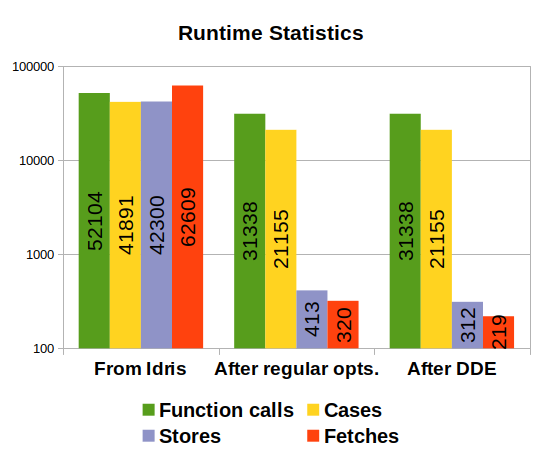
\includegraphics[scale=0.40]{length_rt.png}}
		\end{minipage}
		\hspace{1cm}
		\begin{minipage}{0.45\textwidth}
			\resizebox{\width}{5.5cm}{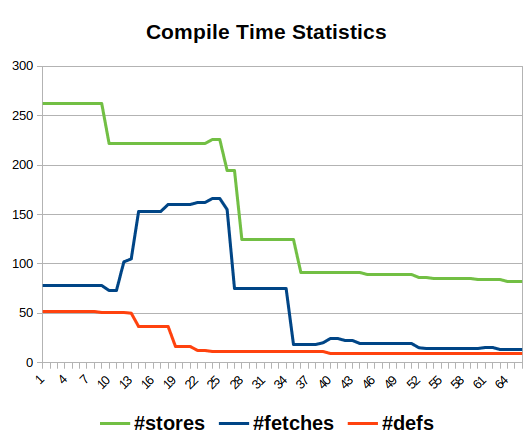
\includegraphics[scale=0.40]{length_ct.png}}
		\end{minipage}
	\end{figure}
	
\end{frame}

\begin{frame}[fragile]
\frametitle{Exact length}
	% no stores & no fetches! (Maybe transformed)
	\begin{figure}
		\hspace{-1cm}
		\begin{minipage}{0.45\textwidth}
			\resizebox{\width}{5.5cm}{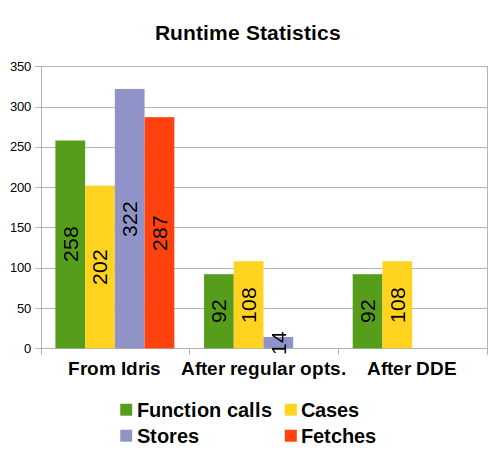
\includegraphics[scale=0.40]{exact_length_rt.png}}
		\end{minipage}
		\hspace{1cm}
		\begin{minipage}{0.45\textwidth}
			\resizebox{\width}{5.5cm}{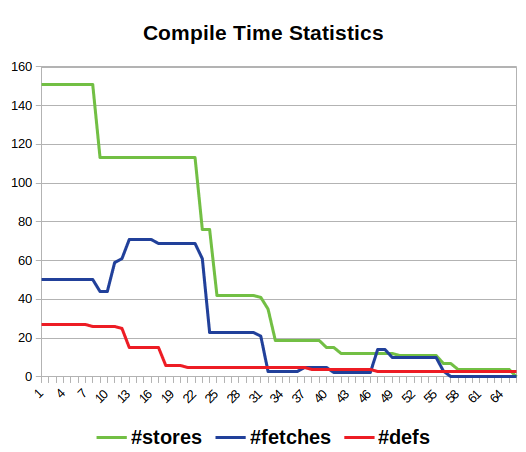
\includegraphics[scale=0.40]{exact_length_ct.png}}
		\end{minipage}
	\end{figure}
\end{frame}

\begin{frame}[fragile]
\frametitle{Reverse}
  % interesting example, but no DDE
  \begin{figure}
  	\hspace{-1cm}
  	\begin{minipage}{0.45\textwidth}
  		\resizebox{\width}{5.5cm}{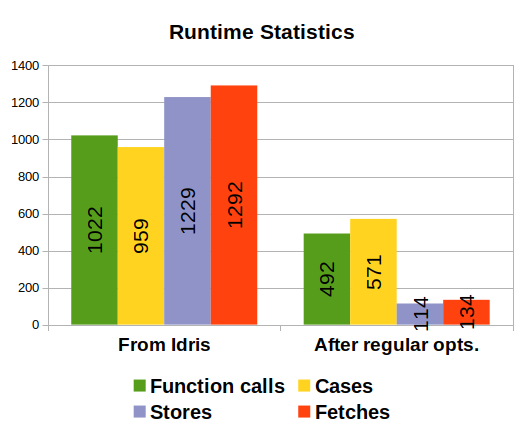
\includegraphics[scale=0.40]{reverse_rt.png}}
  	\end{minipage}
  	\hspace{1cm}
  	\begin{minipage}{0.45\textwidth}
  		\resizebox{\width}{5.5cm}{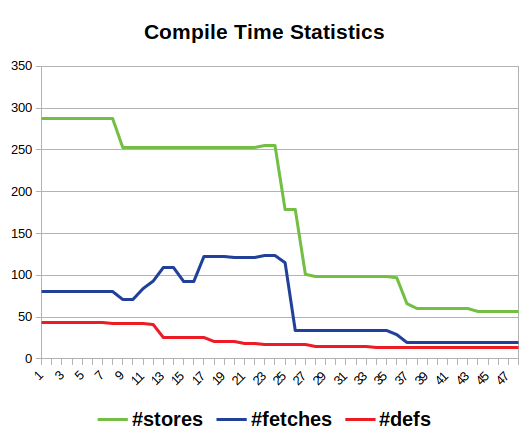
\includegraphics[scale=0.40]{reverse_ct.png}}
  	\end{minipage}
  \end{figure}
\end{frame}

\begin{frame}[fragile]
\frametitle{Type level functions}
  % caveat
  \begin{figure}
  	\hspace{-1cm}
  	\begin{minipage}{0.45\textwidth}
  		\resizebox{\width}{5.5cm}{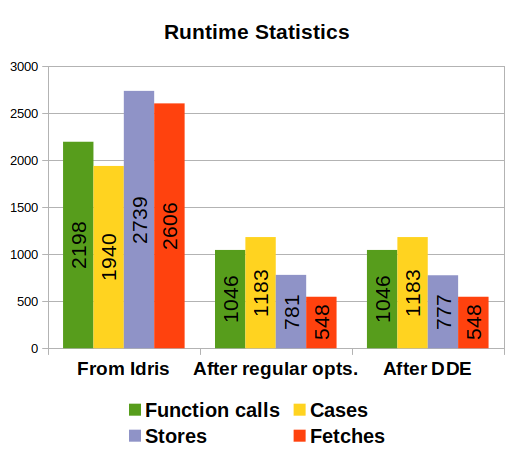
\includegraphics[scale=0.40]{tyfuns_rt.png}}
  	\end{minipage}
  	\hspace{1cm}
  	\begin{minipage}{0.45\textwidth}
  		\resizebox{\width}{5.5cm}{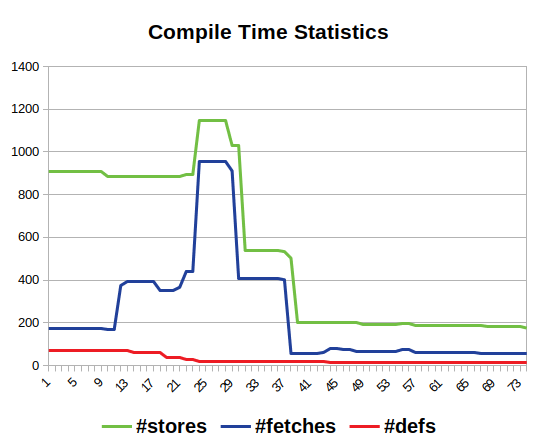
\includegraphics[scale=0.40]{tyfuns_ct.png}}
  	\end{minipage}
  \end{figure}
\end{frame}


\begin{frame}[fragile]
\frametitle{Conclusions}
	\begin{vfitemize}
		\item The optimizer works well:
			\begin{itemize}
				\item the number of stores, fetches, function calls and pattern matches significantly decreased
				\item the structure of the code resembles that of an imperative language
			\end{itemize}
		\item Dead Data Elimination:
			\begin{itemize}
				\item is a bit costly 
				\item is a specific optimization
				\item can completely transform data structures
				\item can trigger further transformations
			\end{itemize}
	\end{vfitemize}
\end{frame}


{
	\usebackgroundtemplate{
\includegraphics[width=\paperwidth]{title.jpg}}%
	\begin{frame}{}
	
	\bigskip\bigskip\bigskip
	
	{\bf\Huge\color{white} THANK YOU}
	
	\bigskip
	
	{\bf\Huge\color{white} FOR YOUR}
	
	\bigskip
	
	{\bf\Huge\color{white} ATTENTION!}
	
\end{frame}
}

% Q&A

\begin{frame}[fragile]
\frametitle{Sparse case optimization}

\begin{center}
	\begin{minipage}{0.40\textwidth}
		\begin{haskellcode}
			<m0>
			v <- eval l
			case v of
			CNil       -> <m1>
			CCons x xs -> <m2>
		\end{haskellcode}
	\end{minipage}
	$\xRightarrow{v \in \{ \text{CCons}\}}$
	\hfill
	\begin{minipage}{0.40\textwidth}
		\begin{haskellcode}
			<m0>
			v <- eval l
			case v of
			CCons x xs -> <m2>
		\end{haskellcode}
	\end{minipage}
\end{center}

\end{frame}


\begin{frame}
\frametitle{Compiled data flow analysis}

\begin{vfitemize}
	\item Analyzing the syntax tree has an interpretation overhead
	\item We can work around this by "compiling" our analysis into an executable program
	\item The compiled abstract program is independent of the AST
	\item It can be executed in a different context (ie.: by another program or on GPU)
	\item After run (iteratively), it produces the result of the given analysis
\end{vfitemize}
\end{frame}






















\begin{frame}

\end{frame}

\begin{frame}[fragile]
	\frametitle{A small functional program}
	
	\begin{haskellcode}
	  main = sum (upto 0 10)
	  
	  upto from to
	    | from > to = []
	    | otherwise = from : upto (from+1) to
	                              
	  sum []     = 0
	  sum (x:xs) = x + sum xs
	\end{haskellcode}
	
\end{frame}



\begin{frame}[fragile]
	\frametitle{Strict control flow}
	
	\begin{minipage}{0.35\textwidth}
		\vspace{-2cm}
		\begin{haskellcode}
			main = sum (upto 0 10)
			
			upto m n
			  | m > n = []
			  | otherwise = m : upto (m+1) n
			
			sum []     = 0
			sum (x:xs) = x + sum xs
		\end{haskellcode}
	\end{minipage}
	\hfill 
	\begin{minipage}{0.6\textwidth}
		\vspace{3cm}
		\begin{figure}[h]
			\centering
			\begin{adjustbox}{scale = 1.4}
				\tikzset{every loop/.style={-{Stealth[scale=1.5]}}}
				
				\begin{tikzpicture}[ node distance = 1cm and 1cm
				, on grid 
				, loop/.append style={-triangle 60}
				]
				
				\node [shape=ellipse,draw=black] (main)                        {main};
				\node [shape=ellipse,draw=black] (sum)  [below left =of main]  {sum};
				\node [shape=ellipse,draw=black] (upto) [below right =of main] {upto};
				
				\path[-{Stealth[scale=1.5]}] 
				(main) edge [] (sum)
				(main) edge [] (upto)
				(sum) edge [loop left] (sum)
				(upto) edge [loop right] (upto);
				
				
				\end{tikzpicture}
			\end{adjustbox}
			\label{control-flow-strict}
		\end{figure}
	\end{minipage}
	
\end{frame}








\begin{frame}[fragile]
\frametitle{Optimized lazy control flow}

\begin{minipage}{0.35\textwidth}
	\vspace{-2cm}
	\begin{haskellcode}
		main = sum (upto 0 10)
		
		upto m n
		  | m > n = []
		  | otherwise = m : upto (m+1) n
		
		sum []     = 0
		sum (x:xs) = x + sum xs
	\end{haskellcode}
\end{minipage}
\hfill 
\begin{minipage}{0.3\textwidth}
	\vspace{1	cm}
	\begin{figure}[h]
		\centering
		\begin{adjustbox}{scale = 1.4}
			\tikzset{every loop/.style={-{Stealth[scale=1.5]}}}
			
			\begin{tikzpicture}[ node distance = 1.3cm and 1cm
			, on grid 
			, loop/.append style={-triangle 60}
			]
			
			\node [shape=ellipse,draw=black]        (main)                  {main};
			\node [shape=ellipse,draw=black]        (sum)  [below =of main] {sum};
			\node [shape=ellipse,draw=black,dashed] (upto) [below =of sum]  {upto};
			
			\path[-{Stealth[scale=1.5]}] 
			(main) edge [] (sum)
			(sum) edge [loop right] (sum)
			(sum) edge [] (upto);
			
			
			\end{tikzpicture}
		\end{adjustbox}
		\label{control-flow-lazy-opt}
	\end{figure}
\end{minipage}

\end{frame}


\begin{frame}
	\frametitle{Goals}
	
	\vspace{-2cm}
	\begin{vfitemize}
		\item We need to handle laziness
		\item We need to optimize across functions
		\item Accomplish both of these for all functional languages
	\end{vfitemize}
	
\end{frame}






\begin{frame}[fragile]
	\frametitle{Properties}
	
	\begin{vfitemize}
		\item Designed for the computer 
		\item Simple syntax, and semantics
		\item Untyped, but we use a typed version (for LLVM)
		\item First order language 
		\item Monadic structure 
		\item Singe Static Assignment property 
		\item Explicit laziness
		\item Global \mintinline{haskell}{eval} (generated)
		\item No unknown function calls
	\end{vfitemize}
\end{frame}



\begin{frame}
	\frametitle{Semantics}
	
	\begin{vfitemize}
		\item C, F, P nodes
		\item Only basic values and pointers can be in nodes
		\item Functions cannot return pointers
			\begin{itemize}
				\item[-] More register usage is exposed
				\item[-] The caller can decide whether the return value should be put onto the heap
			\end{itemize}
		\item \mintinline{haskell}{store},
				  \mintinline{haskell}{fetch},
				  \mintinline{haskell}{update}
		\item Control flow can only diverge and merge at case expressions
	\end{vfitemize}
\end{frame}

\begin{frame}[fragile]
	\frametitle{Laziness in GRIN}
		
	\begin{haskellcode}
    upto m n = 
      (CInt m') <- eval m
      (CInt n') <- eval n
      b' <- _prim_int_gt m' n'
      if b' then
        pure (CNil)
      else
        m1' <- _prim_int_add m' 1
        m1  <- store (CInt m1')
        p   <- store (Fupto m1 n)
        pure (CCons m p)
	\end{haskellcode}
	
\end{frame}










\begin{frame}[fragile]
\frametitle{Dead data elimination}

	\begin{center}
		\begin{minipage}{0.40\textwidth}
			\begin{haskellcode}
				<m0>
				n <- pure (CPair a b)
				(CPair x y) <- pure n
				<m1>
			\end{haskellcode}
		\end{minipage}
		\hfill
		$\xRightarrow{\text{x is dead}}$
		\hfill
		\begin{minipage}{0.35\textwidth}
			\begin{haskellcode}
				<m0>
				n <- pure (CPair b)
				(CPair y) <- pure n
				<m1>
			\end{haskellcode}
		\end{minipage}
	\end{center}

\end{frame}



\begin{frame}
	\frametitle{Analysis types}
	
	\begin{vfitemize}
		\item Whole program analysis\\
		\begin{itemize}
			\item[] The entire program is subject to the analysis
		\end{itemize}
	
		\item Interprocedural program analysis
		\begin{itemize}
			\item[] The analysis is performed across functions
		\end{itemize}
		
		\item Context insensitive program analysis
		\begin{itemize}
			\item Information is not propagated back to the call site
		\end{itemize}
	\end{vfitemize}
\end{frame}



\begin{frame}[fragile]
  \frametitle{Heap-points-to}
  
  \begin{center}
  	\begin{minipage}{0.35\textwidth}
  		\begin{haskellcode}
      grinMain =
        a0 <- pure 5
        n0 <- pure (CNil)
        p0 <- store n0 
        n1 <- pure (CCons a0 p0)
        r  <- case n1 of 
          (CNil) -> 
            pure (CNil)
          (CCons x xs) -> 
            xs' <- fetch xs
            pure xs'
        pure r
  		\end{haskellcode}
  	\end{minipage}
  	\hfill
  	\begin{minipage}{0.48\textwidth}
  		\begin{haskellcode}
  			Heap
  			0 -> {CNil[]}
  			Env
  			a0  -> {T_Int64}
  			n0  -> {CNil[]}
  			n1  -> {CCons[{T_Int64},{0}]}
  			p0  -> {0}
  			r   -> {CNil[]}
  			x   -> {T_Int64}
  			xs  -> {0}
  			xs' -> {CNil[]}
  			Function
  			grinMain :: {CNil[]}
  			
  		\end{haskellcode}
  	\end{minipage}
  \end{center}
  
\end{frame}

\begin{frame}[fragile]
\frametitle{Created-by}

\begin{center}
	\begin{minipage}{0.4\textwidth}
		\begin{haskellcode}
			grinMain =
			  a0 <- pure 5
			  n0 <- pure (CNil)
			  p0 <- store n0 
			  n1 <- pure (CCons a0 p0)
			  r  <- case n1 of 
			    (CNil) -> 
			      pure (CNil)
			    (CCons x xs) -> 
			      xs' <- fetch xs
			      pure xs'
			  pure r
		\end{haskellcode}
	\end{minipage}
	\hfill
	\begin{minipage}{0.40\textwidth}
		\begin{haskellcode}
			Producers
			a0     -> {}
			n0     -> {CNil{n0}}
			n1     -> {CCons{n1}}
			p0     -> {}
			r      -> {CNil{n0}}
			x      -> {}
			xs     -> {}
			xs'    -> {CNil{n0}}
		\end{haskellcode}
	\end{minipage}
\end{center}

\end{frame}


\begin{frame}
\frametitle{Producers and consumers}

\begin{figure}[h]
	\centering
	\begin{adjustbox}{scale = 1.3}
		\begin{tikzpicture}[ node distance = 1cm and 2cm, on grid ]
		
		\node [shape=circle,draw=black] (P1)                 {$P_1$};
		\node [shape=circle,draw=black] (P2) [right =of P1]  {$P_2$};
		\coordinate (Middle) at ($(P1)!0.5!(P2)$);
		\node [shape=circle,draw=black] (C2) [below =of Middle]  {$C_2$};
		\node [shape=circle,draw=black] (C1) [left =of C2]       {$C_1$};
		\node [shape=circle,draw=black] (C3) [right =of C2]      {$C_3$};
		
		\path[-{Stealth[scale=1.5]}] (P1) edge [] (C1)
		(P1) edge [] (C2)
		(P2) edge [] (C2)
		(P2) edge [] (C3);
		
		
		\end{tikzpicture}
	\end{adjustbox}
	\label{fig:producers-and-consumers}
\end{figure}

\end{frame}


\begin{frame}[fragile]
\frametitle{Liveness}

\begin{center}
	\begin{minipage}{0.35\textwidth}
		\begin{haskellcode}
			grinMain =
			  a0 <- pure 5
			  n0 <- pure (CNil)
			  p0 <- store n0 
			  n1 <- pure (CCons a0 p0)
			  r <- case n1 of 
			    (CNil) -> 
			      pure (CNil)
			    (CCons x xs) -> 
			      xs' <- fetch xs
			      pure xs'
			  pure r
		\end{haskellcode}
	\end{minipage}
	\hfill
	\begin{minipage}{0.45\textwidth}
		\begin{haskellcode}
			Heap
			0      -> {CNil[]}
			Env
			a0     -> DEAD
			n0     -> {CNil[]}
			n1     -> {CCons[DEAD,LIVE]}
			p0     -> LIVE
			r      -> {CNil[]}
			x      -> DEAD
			xs     -> LIVE
			xs'    -> {CNil[]}
			Function
			grinMain :: {CNil[]}
		\end{haskellcode}
	\end{minipage}
\end{center}

\end{frame}

\begin{frame}
\frametitle{Results}
\begin{vfitemize}
	\item eval inlinig impact on code size
	\item dead code elimination impact on code size
	\item dead code elimination impact on performance
	\item comparing intra- and interprocedural dead code elimination
		\item how costly they are?
		\item how the resulting codes differ?
	\item how should the transformations be ordered to minimize compilation time, and maximize performance?
	\item how costly are the analyses?
	\item how does the GRIN optimized code compare to GHC's?
\end{vfitemize}
\end{frame}

\begin{frame}
	\frametitle{Summary}
	\begin{vfitemize}
		\item Compiling functional programs has its own challenges
		\item We can make it easier by introducing a new IR
		\item We can perform elaborate dataflow analyses on the IR, then ...
		\item By transforming the code to a more manageable format, we can utilize the already existing infrastructure of LLVM
	\end{vfitemize}
\end{frame}

\end{document}

